% !TEX TS-program = lualatex+se
% !TEX encoding = UTF-8
\documentclass[12pt, a4paper]{book}

% --- USTAWIENIA STRONY ---
\usepackage{geometry}
\geometry{
%	showframe=true,
%	showcrop=true,
	left=15mm,
	right=15mm,
	top=16mm,
	bottom=16mm,
	marginparwidth=0mm,
	marginparsep=0mm
	}
%\usepackage[letterpaper,showframe]{geometry}	
% usuwanie nagłówków/stopek z\,dokumentu
\usepackage[indent=0pt]{parskip} % ustawianie paragrafów
%\setstretch{1.5} % półtorej linii odległości między wierszami
\usepackage{titlesec} % ustawianie nagłówków
%\usepackage{fullpage} % redukcja marginesów
\usepackage{setspace} % odstępy między liniami
\usepackage{enumitem}% listy numerowane
% -----------------------------

%----------- style nagłówków ----------------
\newcommand{\headingone}{\scshape\Large}
\newcommand{\headingtwo}{\large}
\newcommand{\margintext}[1]{\textit{\small #1}}
% przesunięcia poziome
\newcommand{\smallwidth}{\hskip 1em}
\newcommand{\medwidth}{\hskip 3pt}
\newcommand{\largewidth}{\hskip 12pt}
% przesunięcia pionowe
\newcommand{\linespace}{\vskip 6pt}
\newcommand{\paragraphspace}{\vskip 10pt}
\newcommand{\segmentspace}{\vskip 16pt}
\newcommand{\sectionspace}{\vskip 28pt}
%------------------------------------------

% ------- odstępy między wersetami psalmów -------
\newcommand{\itemsp}{0.8}
% --------------------------------------------------
% --- GREGORIO ---	
\usepackage{gregoriotex}
\gresetlinecolor{gregoriocolor}
\gresetheadercapture{annotation}{greannotation}{string}% odczytuje adnotacje nad inicjałem jako ciąg, co pozwala na jego renderowanie
\gresetheadercapture{commentary}{grecommentary}{string}% odczytuje komentarz jako ciąg, co pozwala na jego renderowanie
\grechangedim{commentaryraise}{0.3cm}{scalable} % podnosi komentarz wystarczająco ponad górną linię
\grechangestyle{annotation}{\color{black}\small}% format adnotacji
\grechangestyle{commentary}{\color{gregoriocolor}\small\itshape}% format komentarza
\grechangestyle{abovelinestext}{\color{gregoriocolor}\small\itshape}% format napisu nad liniami
\grechangestyle{initial}{\color{gregoriocolor}\fontsize{36}{36}\selectfont} % zmniejsza wielkość inicjału do bardziej proporcjonalnego rozmiaru (=36pt)
\grechangedim{intersyllablespacenotes}{0.26cm}{scalable}% Minimalna odległość między nutami różnych sylab.

% umieszczenie zawartości składu ich unikalnego argumentu po lewej i prawej stronie każdej linii
\let\grelocalleftbox\localleftbox
\let\grelocalrightbox\localrightbox

%\newcommand{\separator}{\greseparator{3}{40}}
%\newfontface\vectis{VectisMonumentalW01-Regular}
%\def\greinitialformat#1{\fontsize{20}{20}\vectis #1}
% ------------------

%\usepackage[hyperindex=true]{hyperref}% przypisy dolne

%---- usun konflikt między paracol i luacolor ----
%-------- kod poprawiający konflikt między paracol i luacolor ----
\ifluatex
\usepackage{luacolor}
\directlua{
 resetboxcolor = function (head,color)
  for n in node.traverse(head) do
    if 
      node.has_attribute(n,oberdiek.luacolor.getattribute(),
        oberdiek.luacolor.getvalue(token.get_macro("default@color")))
    then 
      node.set_attribute(n,oberdiek.luacolor.getattribute(),color)      
    end
    if n.id == node.id("hlist") or n.id == node.id("vlist") then
     resetboxcolor (n.list,color)
    end
 end
 return head
 end 
}

\protected\def\luacolorresetboxcolor#1{%
  \directlua {local color= tex.getattribute(oberdiek.luacolor.getattribute())
              resetboxcolor (tex.getbox(\the#1),color)}}

\else
\protected\def\luacolorresetboxcolor#1{}
\fi
%------ koniec kodu --------------------------------------
%-----------------------------------------------

% --- SPIS TREŚCI -------
%\usepackage{imakeidx}
%\makeindex[title=Alfabetyczny spis program=texindy,options=-M styl.xdy]
%\usepackage{filecontents}
%\begin{filecontents*}{styl.xdy}
%;;; xindy style file
%(markup-locclass-list :open "\dotfill" :sep "")
%(define-attributes (( "textbf" "default" )) )
%(markup-locref   :attr  "textbf"     :open "\textbf{\hyperpage{" :close "}}")
%(markup-locref   :attr  "textit"     :open "\textit{\hyperpage{" :close "}}")
%(markup-locref   :attr  "textttt"     :open "\textttt{\hyperpage{" :close "}}")
%(markup-locref   :attr  "texttsc"     :open "\texttsc{\hyperpage{" :close "}}")
%(markup-locref   :attr  "default"     :open "\hyperpage{" :close "}")
%\end{filecontents*}
% -------------------------

% ---  Konfiguracja kolumn ---
\usepackage{paracol}
\setcolumnwidth{.49\textwidth, .49\textwidth}
\setlength{\columnseprule}{0.4pt}
\setlength{\columnsep}{.02\textwidth}
\colseprulecolor{red}% wymagany pakiet xcolor
\footnotelayout{m}
% ----------------------------

\makeatletter 
\patchcmd\pcol@hfil
 {\copy\pcol@tempboxa}
 {\luacolorresetboxcolor\pcol@tempboxa\copy\pcol@tempboxa}{}{\fail}
\makeatother
% ----------------------------

\footnotelayout{m}

%% --- UKŁAD DWUKOLUMNOWY Z TŁUMACZENIEM ---
%\usepackage{tcolorbox}
%\newtcolorbox{nutybox}{size=minimal, colback=white, colframe=red, arc=0mm, width=\linewidth, halign=left, valign=center}
%\newtcolorbox{tlumbox}{size=minimal, colback=white, colframe=red, arc=0mm, width=\linewidth, halign=left, valign=top, fontupper=\small\itshape} 
%\newcommand{\nuty}[1]{\begin{nutybox}#1 \end{nutybox}}
%\newcommand{\tlum}[1]{\begin{tlumbox}\tlumacz{#1} \end{tlumbox}}
%% ------------------------------------------------------

\usepackage{Tabbing}
\usepackage{longtable}
\usepackage[savepos]{zref}

% --- CZCIONKI DOKUMENTU ---
\usepackage[latin,polish]{babel}
\usepackage{fontspec}
%\usepackage{times}
%\usepackage[math]{anttor}
%\usepackage{tgtermes}
%\usepackage{mathptmx}
\usepackage{ebgaramond}
\usepackage{libertine}
\defaultfontfeatures{Ligatures=TeX}

%\setmainfont{TeX Gyre Termes}
%\setmainfont{TeX Gyre Heros}
%\setmainfont{Calluna Regular}
\setmainfont{EB Garamond}
%\setmainfont{Bodoni Moda}
%\newfontfamily{\sekfont}{Times New Roman}
\newfontfamily{\sekfont}{Libertinus Serif}
\newcommand\sekcjafont{\fontsize{16}{16}\selectfont \sekfont}

%----- Strona tytułowa -------------
\newfontfamily{\tytfont}{JSL Ancient}
\newcommand\tytulfont[1]{\fontsize{36}{30}\selectfont \tytfont#1\par}
\newcommand\podtytulfont[1]{\fontsize{18}{10}\selectfont \tytfont#1\par}

%\setmainfont[<font features>]{<name of font>} % sets the roman font
%\setsansfont[<font features>]{<name of font>} % sets the sans font
%\setmonofont[<font features>]{<name of font>} % sets the monospace font

% --- KONIEC CZCIONKI DOKUMENTU ---

% --- GRAFIKA I KOLORY ---
\usepackage{xcolor} % kolory
\usepackage{graphicx} % umożliwia import obrazów
\graphicspath{{img/}} % katalog obrazów
\usepackage{pgfornament}% ornamenty graficzne
% --- KONIEC GRAFIKA I KOLORY -----------

% --- KOMENDY WŁASNE ---
\newcommand{\red}[1]{\textcolor{red}{#1}}
\newcommand{\black}[1]{\textcolor{black}{#1}}
% --------------------------------
\newcommand{\tlumacz}[1]{\textit{#1}}
\newcommand{\inicjal}[2]{\textcolor{red}{\LARGE\textbf{#1}}{#2}}
%--------------------------------
\titlespacing*{\chapter}{0pt}{0pt}{5pt}	
\titleformat{\chapter}[hang]{\filcenter\LARGE\scshape\bfseries}{}{0pt}{} % format nagłówków
\titlespacing*{\section}{0pt}{0pt}{0pt}	
\titleformat{\section}[hang]{\filcenter\large\bfseries\scshape}{}{0pt}{} % format nagłówków
\titlespacing*{\subsection}{0pt}{0pt}{0pt}	
\titleformat{\subsection}[hang]{\filcenter\large\scshape}{}{0pt}{} % format podnagłówków

% ----------- RUBRYKA -------------------
\newcommand{\rubryka}[1]{
	\begin{spacing}{0.8}
	\begin{center}
		\parbox{0.9\textwidth}{\centering\textcolor{red}{\small\textit{#1}}}
	\end{center}
	\end{spacing}
	\linespace}
% ------- rubryka w tekście ---------------	
\newcommand{\rub}[1]{
	\textcolor{red}{\small\textit{#1}}
	}
% ----------- SEKCJA --------------------
% -----------------------------------------
%\renewcommand\fbox{\fcolorbox{red}{white}}% czerwona ramka fbox-a
\newcommand{\sekcja}[2]{
	\begin{spacing}{0.6}
	\begin{center}
		\section*{#1}
		\linespace
		\begin{minipage}{\linewidth}
			\red{\small\textit{#2}}
		\end{minipage}
	\end{center}	
	\end{spacing}
	\paragraphspace}
%-----------------------------------------
\newcommand{\subsekcja}[1]{
	\begin{spacing}{0.6}
		\subsection*{#1}
		\linespace
	\end{spacing}
	\paragraphspace}
%------------DEKOR ---------------------
\newcommand{\dekor}[2]{
	\begin{center}
		\vspace*{\fill}
		\includegraphics[width=#1\textwidth]{#2}
		\vspace*{\fill}
	\end{center}}
%------- Zarządzanie wersami w psalmach z tlumaczeniem -------------------------
\newcounter{licznik}
\newcommand{\licznikZero}{\setcounter{licznik}{0}}% zeruj licznik
\newcommand{\licznikUp}{\refstepcounter{licznik}}% zwiększ licznik 
\licznikZero
\newcommand{\BeginParallel}{\begin{spacing}{0.9} \begin{paracol}{2} \licznikZero}
\newcommand{\lat}[1]{\selectlanguage{latin}\ensurevspace{2\baselineskip}\begin{minipage}[t]{\linewidth}\ifnum \value{licznik}>0 \licznikUp \thelicznik .~{#1}\par \else \licznikUp{#1}\par \fi \end{minipage}\switchcolumn}
\newcommand{\latN}[1]{\selectlanguage{latin}\ensurevspace{2\baselineskip}\begin{minipage}[t]{\linewidth}{#1}\par\end{minipage}\switchcolumn}% kolumna bez numeracji wersów
\newcommand{\pol}[1]{\selectlanguage{polish}\begin{minipage}[t]{\linewidth}{#1}\par\end{minipage}\switchcolumn*}
\newcommand{\EndParallel}{\end{paracol} \end{spacing}}

% --- ZNAKI SPECJALNE ---
% 
%\newcommand <c>†</c>
% --------------------------

\begin{document}
\pagestyle{plain}	
\large

\setlength{\parindent}{0pt}
\gresetbracerendering{font}

\pagenumbering{gobble} % nie jest wyprowadzany żaden numer strony, chociaż numer jest nadal resetowany. Odniesienia do tej strony również są puste.
%% --------------------------------- STRONA TYTUŁOWA  ---------------------------------
\begin{center}
	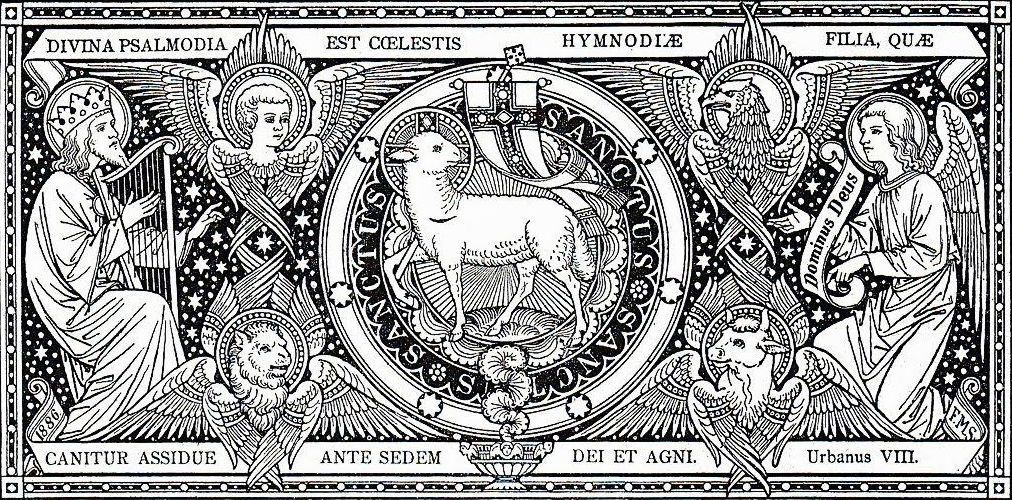
\includegraphics[width=1.0\linewidth]{divina_psalmodia.jpg}
	\vfill
	\podtytulfont{}
	\tytulfont{COMPLETORIUM}
	\vfill
	\large\textit{Liber usualis, Solesmes, 1961, p.1400}
\end{center}
\newpage
\pagenumbering{arabic}
%% --------------------------------  MODLITWY WSTĘPNE --------------------------------
\sekcja{Modlitwa przygotowawcza}{Całość odmawia się po cichu i~w~pozycji klęczącej. Na pierwsze słowa kreśli się znak krzyża na ustach. }
\sectionspace
%% ----------------- Modlitwy wstępne ----------
\BeginParallel
	\latN{\inicjal{A}{péri},\red{+}Dómine, os meum ad benedicéndum nomen sanctum tuum: munda quoque cor meum ab ómnibus vanis, pervérsis et aliénis cogitatiónibus; intelléctum illúmina, afféctum inflámma, ut digne, atténte ac devóte hoc Offícium recitáre váleam, et exaudíri mérear ante conspéctum divínæ Majestátis tuæ. Per Christum Dóminum nostrum. Amen.}
	\pol{\tlumacz{\inicjal{O}{twórz},\red{+}Panie, usta moje, dla błogosławienia świętego imienia Twego: oczyść także serce moje od wszelkich myśli próżnych, przewrotnych i~niewłaściwych; oświeć rozum, rozpal uczucie, abym godnie, uważnie i~pobożnie mógł odmówić to oficjum, i~zasłużył na wysłuchanie przed obliczem Twego Boskiego majestatu. Przez Chrystusa, Pana naszego. Amen.}}
  	\latN{\inicjal{D}{ómine}, in unióne illíus divínæ intentiónis, qua ipse in terris laudes Deo persolvísti, hanc tibi Horam persólvo.}
	\pol{\tlumacz{\inicjal{P}{anie}, w~zjednoczeniu z~tą Boską intencją, z~którą Ty sam, na ziemi będąc, chwałę Bogu zanosiłeś, Tobie tę godzinę zanoszę.}}
\EndParallel% hanc - jedna godzina, has - kilka godzin
\dekor{0.4}{amdg800x533.jpg}
\newpage
%% --------------------------------  INCIPIT --------------------------------
\large
\setstretch{1.1} 
\sekcja{Incipit}{Wszyscy wstają. Lektor wychodzi na środek, przyklęka i skłaniając się w kierunku kapłana prosi o błogosławieństwo. W~przypadku braku kapłana: "Jube Domine benedicere". Błogosławieństwo - odpowiada kapłan lub pod jego nieobecność hebdomadariusz}
\linespace
% Jube domne / Noctem
\gresetinitiallines{0}\gabcsnippet{(c3) <c><sp>V/</sp>.</c> Ju([alt:Lector incipit]h)be(h) dom(h)ne(g'_) be(h)ne(h)di(h)ce(d)re(f.)(::)}
\linespace
\gresetinitiallines{0}\gabcsnippet{(c3) Noc([alt:Hebdomadarius - benedictio]h)tem(h) qui(h)ét(h)am(h) et(h) fi(h)nem(g) per(f)féc(h)tum(h.;) con(h)cé(h)dat(h) no(h)bis(h) Do(h)mi(h)nus(h) o(h)mni(h)po(d)tens(d.::)}
\gresetinitiallines{0}\gabcsnippet{(c3) <c><sp>R/</sp>.</c> A(g.)men(h.::)}
\linespace
%% --------------------------------  LECTIO BREVIS --------------------------------
% Lectio brevis - Completorium
\gresetinitiallines{1}\grecommentary{1 Petri 5,8-9}\gabcsnippet{(c3) Frá([alt:Lector - lectio brevis]h)tres:(h.)(,) Só(h)bri(h)i(h) e(h)stó(h)te(h), et(h) vi(h)gi(h)lá(h)te:(f.;) qui(h)a(h) a(h)dver(h)sá(h)ri(h)us(h) vés(h)ter(h) diá(h)bo(h)lus,(h'_)(,) tam(h)quam(h) lé(h)o(h) rú(h)gi(h)ens,(h'_)(,) cír(h)cu(h)it(h), quaé(h)rens(g) quem(f) dé(h)vo(h)ret:(h.;) cú(h)i(h) re(h)sí(h)sti(h)te(h) fór(h)tes(h) in(h) fí(h.)de.(d.:) Tu(h) au(g)tem(f) Dó(h)mi(h)ne(h._), mi(h)se(h)ré(h)re(h) nó(h.)bis.(d.::) <c><sp>R/</sp>.</c> De(h)o(h) grá(h)ti(d)as.(d.::)}

\linespace
% Adiutorium nostrum
\gresetinitiallines{0}\gabcsnippet{(c3) <c><sp>V/</sp>.</c> Ad(h[alt:Hebdomadarius])ju(h)to(h)ri(h)um(h) nos(h)trum(h) in(h) no(h)mi(h)ne(h) Do(h)mi(f)ni(f) (::)}
\gresetinitiallines{0}\gabcsnippet{(c3) <c><sp>R/</sp>.</c> Qui fe(h[alt:Chorus respondet])cit(h) cae(h)lum(h) et(h) ter(h)ram.(f') (::)}% głosem niskim
\inicjal{P}{ater} noster... \rub{(cicho, następnie Hebdomadariusz spowiada się głosem prostym i przyciszonym)}\\
\rub{Chór odpowiada:}\\
\inicjal{M}{isereátur} túi omnípotens Deus, et dimíssis peccátis túis, perdúcat te ad vitam ætérnam. \red{\Rbar.}~Amen.\\
\rub{Chór spowiada się:}\\
\inicjal{C}{onfíteor} Deo omnipoténti, beátæ Maríæ semper Vírgini, beáto Michaéli Archángelo, beáto Joánni Baptístæ, sanctis Apóstolis Petro et Paulo, et ómnibus Sanctis, quia peccávi nimis, cogitatióne, verbo et ópere: \rub{bijąc się w piersi} mea culpa, mea culpa, mea máxima culpa. Ídeo precor beátam Maríam semper Vírginem, beátum Michaélem Archángelum, beátum Joánnem Baptístam, sanctos Apóstolos Petrum et Paulum, et omnes Sanctos, oráre pro me ad Dóminum Deum nostrum.\\
\rub{Hebdomadariusz odpowiada:}\\
\inicjal{M}{isereátur} véstri omnípotens Deus, et dimíssis peccátis véstris, perdúcat vos ad vitam ætérnam. \red{\Rbar.}~Amen.\\
\inicjal{I}{ndulgéntiam}, \red{+} absolutiónem et remissiónem peccatórum nostrórum tríbuat nobis omnípotens et miséricors Dóminus. \red{\Rbar.}~Amen.\\
% Adiutorium nostrum
\gresetinitiallines{0}\gabcsnippet{(c3) <c><sp>V/</sp>.</c> Con(h[alt:Hebdomadarius])vér(h)te(h) nos(h) Déus(h) sa(h)lu(h)tá(g)ris(f) nó(h)ster(h) (::)}
\gresetinitiallines{0}\gabcsnippet{(c3) <c><sp>R/</sp>.</c> Et(h[alt:Chorus respondet]) a(h)vér(h)te(h) í(h)ram(h)  tú(h)am(g) a(f) nó(h)bis.(h) (::)}% głosem uniesionym, znak krzyża na piersi
\linespace
\grechangedim{intersyllablespacenotes}{0.02cm}{scalable}% Minimalna odległość między nutami różnych sylab.
\gresetinitiallines{1}\greannotation{\Vbar.}\gabcsnippet{(c3) DE(h[alt:Hebdomadarius])us(h'_) (,) in(h) ad(h)ju(h)tó(i)ri(h)um(h) me(h)um(h'_) in(h)tén(g)de.(h.) (::)
<c><sp>R/</sp>.</c> Dó(h[alt:Chorus respondet])mi(h)ne(h'_) (,) ad(h) ad(h)ju(h)ván(h)dum(h) me(h'_) fe(h)stí(g)na.(h.) (:) Gló(h)ri(h)a(h) Pa(h)tri,(h) et(h) Fí(h)li(h)o,(h'_) (,) et(h) Spi(h)rí(h)tu(h)i(h) San(g)cto.(h.) (:) Sic(h)ut(h) e(h)rat(h) in(h) prin(h)cí(h)pi(h)o,(h) et(h) nunc,(h) et(h) sem(h)per,(h.) (,) et(h) in(h) saé(h)cu(h)la(h) sae(h)cu(h)ló(h)rum.(h) A(g)men.(h.) (;) Al(h[alt:per annum])le(i)lú(hg~){ia. }(g.) (::) <i>Vel:</i>() <alt>a Septuagesima usque ad Pascha</alt> Laus(h) ti(h)bi(h) Dó(h)mi(h)ne(h'_) Rex(h) ae(h)tér(h)nae(i) gló(h')ri(h)ae.(g.) (::)}
\grechangedim{intersyllablespacenotes}{0.26cm}{scalable}% Minimalna odległość między nutami różnych sylab.
%% --------------------------------  PSALMI --------------------------------
\sectionspace
\sekcja{Psalmi}{}
\subsekcja{Feria sexta}{}
\gresetinitiallines{1}\greannotation{Ant.}\greannotation{7. c}\gabcsnippet{(c3) VO(i')ce(g) me(iv.jki)a(i'_[oh:h]) <c>‡</c> (::)}
\red{\normalsize{Psalm 76(2-13) [1]}\linespace}
\greannotation{Psalm}\greannotation{76(2-13)}\gabcsnippet{(c3)Vo(hg)ce(hi) me(i)a(i) ad(i) Dó(i)mi(i)<b>num</b>(k jr) cla(j)<b>má</b>(i jr)vi:(j.) <c><v>\greheightstar</v></c>(:) vo(i)ce(i) me(i)a(i) ad(i) De(i)um,(i) et(i) in(i)<b>tén</b>(j ir)dit(i) <b>mi</b>(h hr)hi.(gh.. ) (::)()
<i> Flex:</i>()  ex(i)qui(i)sí(i)vi(h.), <c>†</c>(::)}
\begin{enumerate}[start=2, leftmargin=*]
\begin{spacing}{\itemsp}
\item In die tribulatiónis meæ Deum exquisívi,~† mánibus meis nocte contra eum:~* et non sum decéptus.
\item Rénuit consolári ánima mea:~† memor fui Dei, et delectátus sum, et exercitátus sum:~* et defécit spíritus meus.
\end{spacing}
\end{enumerate}
\gresetinitiallines{0}\gabcsnippet{(c3)4. An(i)ti(i)ci(i)pa(i)vé(i)runt(i) vi(i)gí(i)li(i)as(i) <b>ó</b>(k)cu(jr)li(j) <b>me</b>(i jr)i:(j.) <c><v>\greheightstar</v></c>(:) tur(i)bá(i)tus(i) sum,(i) et(i) non(i) <b>sum</b>(j ir) lo(i)<b>cú</b>(h hr)tus.(gh..) (::)}
\begin{enumerate}[start=5, leftmargin=*]
\begin{spacing}{\itemsp}
\item Cogitávi dies antíquos:~* et annos ætérnos in mente hábui.
\item Et meditátus sum nocte cum corde meo,~* et exercitábar, et scopébam spíritum meum.
\item Numquid in ætérnum projíciet Deus:~* aut non appónet ut complacítior sit adhuc?
\item Aut in finem misericórdiam suam abscíndet,~* a generatióne in generatiónem?
\item Aut obliviscétur miseréri Deus:~* aut continébit in ira sua misericórdias suas?
\item Et dixi: Nunc cœpi:~* hæc mutátio déxteræ Excélsi.
\item Memor fui óperum Dómini:~* quia memor ero ab inítio mirabílium tuórum.
\item Et meditábor in ómnibus opéribus tuis:~* et in adinventiónibus tuis exercébor.
\item Glória Patri, et Fílio,~* et Spirítui Sancto.
\item Sicut erat in princípio, et nunc, et semper,~* et in sǽcula sæculórum. Amen.
\end{spacing}
\end{enumerate}
\red{\normalsize{Psalm 76(14-21) [2]}\linespace}
\gresetinitiallines{1}\greannotation{Psalm}\greannotation{76(14-21)}\gabcsnippet{(c3)De(hg)us,(hi) in(i) sanc(i)to(i) vi(i)a(i) tu(i)a: <c>†</c>(h.) quis(i) De(i)us(i) ma(i)gnus(i) sic(i)ut(i) <b>De</b>(k jr)us(j) <b>nos</b>(i jr)ter?(j.) <c><v>\greheightstar</v></c>(:) tu(i) es(i) De(i)us(i) qui(i) fa(i)cis(i) <b>mi</b>(j ir)ra(i)<b>bí</b>(h)li(hr)a.(gh..) (::)}
\begin{enumerate}[start=2, leftmargin=*]
\begin{spacing}{\itemsp}
\item Notam fecísti in pópulis virtútem tuam:~* redemísti in bráchio tuo pópulum tuum fílios Jacob et Joseph.
\item Vidérunt te aquæ, Deus, vidérunt te aquæ:~* et timuérunt et turbátæ sunt abýssi.
\item Multitúdo sónitus aquárum:~* vocem dedérunt nubes.
\item Etenim sagíttæ tuæ tránseunt:~* vox tonítrui tui in rota.
\item Illuxérunt coruscatiónes tuæ orbi terræ:~* commóta est, et contrémuit terra.
\item In mari via tua, et sémitæ tuæ in aquis multis:~* et vestígia tua non cognoscéntur.
\item Deduxísti sicut oves pópulum tuum,~* in manu Móysi et Aaron.
\item Glória Patri, et Fílio,~* et Spirítui Sancto.
\item Sicut erat in princípio, et nunc, et semper,~* et in sǽcula sæculórum. Amen.
\end{spacing}
\end{enumerate}
\newpage
\red{\normalsize{Psalm 85 [3]}\linespace}
\gresetinitiallines{1}\greannotation{Psalm}\greannotation{85)}\gabcsnippet{(c3)In(hg)clí(hi)na,(i) Dó(i)mi(i)ne,(i) au(i)rem(i) tu(i)am,(i) <b>et</b>(k jr) ex(j)<b>áu</b>(i)di(jr) me:(j.) <c><v>\greheightstar</v></c>(:) quón(i)i(i)am(i) in(i)ops,(i) et(i) <b>pau</b>(j)per(ir) sum(i) <b>e</b>(h hr)go.(gh..) (::) ()
<i>Flex:</i>()  to(i)ta(i) di(i)e:(h.) <c>†</c>(::)}
\begin{enumerate}[start=2, leftmargin=*]
\begin{spacing}{\itemsp}
\item Custódi ánimam meam, quóniam sanctus sum:~* salvum fac servum tuum, Deus meus, sperántem in te.
\item Miserére mei, Dómine, quóniam ad te clamávi tota die:~† lætífica ánimam servi tui,~* quóniam ad te, Dómine, ánimam meam levávi.
\item Quóniam tu, Dómine, suávis et mitis:~* et multæ misericórdiæ ómnibus invocántibus te.
\item Auribus pércipe, Dómine, oratiónem meam:~* et inténde voci deprecatiónis meæ.
\item In die tribulatiónis meæ clamávi ad te:~* quia exaudísti me.
\item Non est símilis tui in diis, Dómine:~* et non est secúndum ópera tua.
\item Omnes gentes quascúmque fecísti, vénient, et adorábunt coram te, Dómine:~* et glorificábunt nomen tuum.
\item Quóniam magnus es tu, et fáciens mirabília:~* tu es Deus solus.
\item Deduc me, Dómine, in via tua,~† et ingrédiar in veritáte tua:~* lætétur cor meum ut tímeat nomen tuum.
\item Confitébor tibi, Dómine, Deus meus, in toto corde meo,~* et glorificábo nomen tuum in ætérnum.
\item Quia misericórdia tua magna est super me:~* et eruísti ánimam meam ex inférno inferióri.
\item Deus iníqui insurrexérunt super me,~† et synagóga poténtium quæsiérunt ánimam meam:~* et non proposuérunt te in conspéctu suo.
\item Et tu, Dómine, Deus miserátor et miséricors,~* pátiens, et multæ misericórdiæ, et verax.
\item Réspice in me, et miserére mei,~† da impérium tuum púero tuo:~* et salvum fac fílium ancíllæ tuæ.
\item Fac mecum signum in bonum,~† ut vídeant qui odérunt me, et confundántur:~* quóniam tu, Dómine, adjuvísti me, et consolátus es me.
\item Glória Patri, et Fílio,~* et Spirítui Sancto.
\item Sicut erat in princípio, et nunc, et semper,~* et in sǽcula sæculórum. Amen.
\end{spacing}
\end{enumerate}
\gresetinitiallines{1}\greannotation{Ant.}\greannotation{7. c}\gabcsnippet{(c3) VO(i')ce(g) me(iv.jki)a(i'_[oh:h]) (,)<c>‡</c> ad(i) Dó(i')mi(g)num(h_i) cla(f')má(e)vi,(e.) (;) ne(h_)que(h') ob(h)li(h)vi(f')scé(h)tur(g'_[oh:h]) (,) mi(f)se(e)ré(fh)ri(g) De(e.)us.(e.) (::)}
%% --------------------------------  HYMNUS --------------------------------
\newpage
\sekcja{Hymnus}{}% wszyscy wstają, hymn śpiewany na zmiany, hebdomadariusz śpiewa Tu autem
\subsekcja{In Feriis et Festis Simplicibus per Annum}{}
\gresetinitiallines{1}\greannotation{Hymn.}\greannotation{8.}\gabcsnippet{(c4) TE(h) lu(j')cis(j) an(j)te(j) tér(k')mi(j)num,(i) (,) Re(h)rum(h') Cre(h)á(h)tor,(h) pó(i')sci(h)mus,(g.) (;) Ut(i) pro(h') tu(g)a(g) cle(f)mén(g')ti(h)a,(h) (,) Sis(j) prae(j')sul(j) et(j) cu(h)stó(i')di(h)a.(g.) 2.(::) Pro(h)cul(j') re(j)cé(j)dant(j) só(k')mni(j)a,(i) (,) Et(h) nó(h')cti(h)um(h) phan(h)tá(i')sma(h)ta:(g.) (;) Ho(i)stém(h')que(g) no(g)strum(f) cóm(g')pri(h)me,(h) (,) Ne(j) pol(j')lu(j)án(j)tur(h) cór(i')po(h)ra.(g.) 3.(::) Prae(h)sta,(j') Pa(j)ter(j) pi(j)ís(k')si(j)me,(i) (,) Pa(h)trí(h')que(h) com(h)par(h) U(i')ni(h)ce,(g.) (;) Cum(i) Spí(h')ri(g)tu(g) Pa(f)rá(g')cli(h)to,(h) (,) Re(j)gnans(j') per(j) o(j)mne(h) saé(i')cu(h)lum.(g.) (::) A(ghg)men.(fg..) (::)}
\subsekcja{In Dominicis et minoribus Festis per Annum}{}
\gresetinitiallines{1}\greannotation{Hymn.}\greannotation{8.}\gabcsnippet{(c4) TE(g) lu(i')cis(h) an(j)te(j) tér(j')mi(i)num,(h) (,) Re(h)rum(j') Cre(j)á(j)tor,(g) pó(h')sci(g)mus,(f.) (;) Ut(h) pro(h') tu(g)a(j) cle(i)mén(h')ti(g)a,(hih') (,) Sis(h) prae(h')sul(g) et(f) cu(g)stó(h')di(g)a.(g.) (::) 
2. Pro(g)cul(i') re(h)cé(j)dant(j) só(j')mni(i)a,(h) (,) Et(h) nó(j')cti(j)um(j) phan(g)tás(h')ma(g)ta :(f.) (;) Ho(h)stém(h')que(g) no(j)strum(i) cóm(h')pri(g)me,(hih') (,) Ne(h) pol(h')lu(g)án(f)tur(g) cór(h')po(g)ra.(g.) (::) 3. Prae(g)sta,(i') Pa(h)ter(j) pi(j)ís(j')si(i)me,(h) (,) Pa(h)trí(j')que(j) com(j)par(g) U(h')ni(g)ce,(f.) (;) Cum(h) Spí(h')ri(g)tu(j) Pa(i)rá(h')cli(g)to,(hih') (,) Re(h)gnans(h') per(g) o(f)mne(g) saé(h')cu(g)lum.(g.) (::)
A(ghg)men.(fg..) (::)}
%% --------------------------------  CAPITULUM --------------------------------
\sectionspace
\sekcja{Capitulum Responsorium Versus}{}
\subsekcja{Per Annum}{}
\gresetinitiallines{1}\greannotation{Cap.}\greannotation{6.}\gabcsnippet{(c3)Tu(h) au(h)tem(h) in(h) no(h)bis(h) es,(h) Dó(h)mi(f)ne,(f.) (,) et(h) no(h)men(h) sanc(h)tum(h) tu(h)um(h) in(h)vo(h)cá(h)tum(g) est(f) su(h)per(h) nos:(h.) (,) ne(h) de(h)re(h)lín(h)quas(h) nos,(h) Dó(h)mi(h)ne,(h) De(h)us(h) nos(f)ter.(ef..) (::) De(h)o(h) gra(f)ti(e)as.(ef..) (::)}
\gresetinitiallines{0}\gabcsnippet{(c3) <c><sp>V/</sp>.</c> Cus(f)tó(f)di(f) nos,(f) Dó(f)mi(f)ne,(f) ut(f) pu(f)píl(f)lam(f) ó(f)cu(f)li.(e_' fEDCded.) (::)}
\gresetinitiallines{0}\gabcsnippet{(c3) <c><sp>R/</sp>.</c> Sub(f) um(f)bra(f) a(f)lá(f)rum(f) tu(f)á(f)rum(f) pró(f)te(f)ge(f) nos.(e_' fEDCded.) (::)}
\gresetinitiallines{1}\greannotation{Resp.}\greannotation{6.}\gabcsnippet{(c4) IN(f) ma(f)nus(f) tu(fg)as(g) Dó(gf)mi(g)ne,(gh..) *(;)  Com(h')mén(f)do(gh) spí(g)ri(fd)tum(fg) me(g.)um.(f.) (::) In(f) ma(f)nus.(f) (::) 
<sp>V/</sp>. Red(h)e(h)mí(ixhi)sti(h) nos(h) Dó(gh)mi(g)ne,(g'_[oh:h]) (,) De(h)us(g') ve(g)ri(gf)tá(g)tis.(gh..) (::) * Com(h')mén(f)do.(gh) (::) 
<sp>V/</sp>. Gló(h)ri(h)a(h) Pa(ixhi)tri,(h'_) (,) et(h) Fí(gh)li(g)o,(g'_[oh:h]) (,) et(g) Spi(g)rí(h')tu(g)i(f') San(g)cto.(gh..) (::) In(f) ma(f)nus.(f) (::) (f+)}
%% --------------------------------  CANTICUM --------------------------------
\sectionspace
\sekcja{Canticum: Nunc dimittis}{}
\gresetinitiallines{1}\greannotation{Ant.}\greannotation{3. a}\gabcsnippet{(c4) SAl(g)va(hj) nos,(j.) (::)}
\gresetinitiallines{1}\greannotation{Cant.}\gabcsnippet{(c4)Nunc(g) di(hj)mít(j)tis(j) ser(j)vum(j) <b>tu</b>(k)um,(j) <b>Dó</b>(j)<b>mi</b>(ih)ne,(j.) <c><v>\greheightstar</v></c>(:) se(j)cún(j)dum(j) ver(j)bum(j) tu(j)um(j) <i>in</i>(h) <b>pa</b>(j)ce:(i.) (::)
<c>2. </c>Qui(g)a(hj) vi(j)dé(j)runt(j) <b>ó</b>(k)cu(j)li(j) <b>me</b>(ih)i(j.) <c><v>\greheightstar</v></c>(:) sa(j)lu(j)tá(j)<i>re</i>(h) <b>tu</b>(j)um,(i.) (::)
<c>3. </c><b>Quod</b>(k) pa(j)<b>rás</b>(ih)ti(j.) <c><v>\greheightstar</v></c>(:) an(j)te(j) fá(j)ci(j)em(j) óm(j)ni(j)um(j) po(j)<i>pu</i>(h)<b>ló</b>(j)rum,(i.) (::)
<c>4. </c>Lu(g)men(hj) ad(j) re(j)ve(j)la(j)ti(j)<b>ó</b>(k)nem(j) <b>Gén</b>(j)<b>ti</b>(ih)um,(j.) <c><v>\greheightstar</v></c>(:) et(j) gló(j)ri(j)am(j) ple(j)bis(j) tu(j)<i>æ</i>(h) <b>Is</b>(j)ra(j)ël.(i.) (::)
<c>5. </c>Gló(g)ri(hj)a(j) <b>Pa</b>(k)tri,(j) et(j) <b>Fí</b>(j)<b>li</b>(ih)o,(j.) <c><v>\greheightstar</v></c>(:) et(j) Spi(j)rí(j)tu(j)<i>i</i>(h) <b>Sanc</b>(j)to.(i.) (::)
<c>6. </c>Sic(g)ut(hj) e(j)rat(j) in(j) prin(j)cí(j)pi(j)o,(j) et(j) <b>nunc</b>,(k) et(j) <b>sem</b>(ih)per,(j.) <c><v>\greheightstar</v></c>(:) et(j) in(j) sǽ(j)cu(j)la(j) sæ(j)cu(j)ló(j)<i>rum</i>.(h) <b>A</b>(j)men.(i.) (::)}
\gresetinitiallines{1}\greannotation{Ant.}\greannotation{3. a}\gabcsnippet{(c4) SAl(g)va(hj) nos,(j.) Dó(jk)mi(j)ne,(ji) vi(h)gi(i')lán(h)tes,(g.) (;) cu(g)stó(i')di(j) nos(k') dor(j)mi(h')én(j)tes :(i.) (;) ut(i) vi(g')gi(i)lé(k')mus(j) cum(h') Chri(j)sto,(i_[uh:l]j) (,) et(h) re(h)qui(h)e(h)scá(gf)mus(gh) in(gf) pa(e.)ce.(e.) (::) <i>T. P.</i> Al(g)le(gf)lú(e.){ia}.(e.) (::)}
%% --------------------------------  ORATIO --------------------------------
\sectionspace
\sekcja{Oratio}{}
\sectionspace
\input{include/dominus_vobiscum}
Orémus.
\incipit{V}{ísita}, quǽsumus, Dómine, habitatiónem istam, et omnes insídias inimíci ab ea lónge repélle: Ángeli tui sancti hábitent in ea, qui nos in pace custódiant; et benedíctio tua sit super nos semper.
Per Dóminum nostrum Jesum Christum, Fílium tuum: qui tecum vivit et regnat in unitáte Spíritus Sancti, Deus, per ómnia sǽcula sæculórum.
\red{\Rbar.}~Amen.
\input{include/dominus_vobiscum}
%% --- Benedicamus completorium ---
\gabcsnippet{(f3) <c><sp>V/</sp>.</c> (c3) <sp>V/</sp>. Be(h')ne(h)di(h)cá(hi)mus(i') Dó(i)mi(i)no.(ivHG.) (::) 
<sp>R/</sp>. De(i)o(i') grá(i)ti(i)as.(ivHG.) (::) }
%% --- End Benedicamus ---
%% --------------------------------  CONCLUSIO --------------------------------
\sectionspace
\sekcja{Conclusio}{}










\newpage
\pagenumbering{gobble} % nie jest wyprowadzany żaden numer strony, chociaż numer jest nadal resetowany. Odniesienia do tej strony również są puste.
%% --- Modlitwy końcowe ---
\sekcja{Modlitwy końcowe}{Odmawia się po cichu w~pozycji klęczącej jako dziękczynienie po oficjum. Tym, którzy będą z~oddaniem na kolanach odmawiać poniższe modlitwy, papież Leon~X udzielił odpustu za te uchybienia i~przewinienia, które być może popełnili z~powodu ludzkiej słabości podczas odmawiania Oficjum.}
\paragraphspace
% Modlitwy końcowe: Sacrosanctae, Pater noster, Ave Maria
\BeginParallel
	\latN{\inicjal{S}{acrosánctæ} et indivíduæ Trinitáti, crucifíxi Dómini nostri Jesu Christi humanitáti, beatíssimæ et gloriosíssimæ sempérque Vírginis Maríæ fœcúndæ integritáti, et ómnium Sanctórum universitáti sit sempitérna laus, honor, virtus et glória ab omni creatúra, nobísque remíssio ómnium peccatórum, per infiníta sǽcula sæculórum. Amen.} 
	\pol{\inicjal{N}{ajświętszej} i~niepodzielnej Trójcy, człowieczeństwu ukrzyżowanego Pana naszego Jezusa Chrystusa, płodnemu dziewictwu błogosławionej i~najchwalebniejszej zawsze Dziewicy Maryi oraz wspólnocie wszystkich świętych niech będzie wieczna chwała, cześć, moc i~sława od wszelkiego stworzenia, a~nam odpuszczenie wszystkich grzechów, przez nieskończone wieki wieków. Amen.}
	\latN{\red{\Vbar.}~Beáta viscera Mariæ Virginis quæ portavérunt ætérni Patris Filium.\\ \red{\Rbar.}~Et beáta úbera quæ lactavérunt Christum Dóminum.}
	\pol{\red{\Vbar.}~Błogosławione łono Maryi Dziewicy, które nosiło Syna Ojca przedwiecznego.\\ \red{\Rbar.}~I~błogosławione piersi, które karmiły Chrystusa Pana.}
	\latN{\inicjal{P}{ater} noster, qui es in cælis, sanctificétur nomen tuum: advéniat regnum tuum: fiat volúntas tua, sicut in cælo et in terra. Panem nostrum quotidiánum da nobis hódie: et dimítte nobis débita nostra, sicut et nos dimíttimus debitóribus nostris: et ne nos indúcas in tentatiónem: sed líbera nos a malo. Amen}
	\pol{\inicjal{O}{jcze} nasz, któryś jest w niebie święć się imię Twoje; przyjdź królestwo Twoje; bądź wola Twoja jako w niebie tak i~na ziemi; chleba naszego powszedniego daj nam dzisiaj; i~odpuść nam nasze winy, jako i~my odpuszczamy naszym winowajcom; i~nie wódź nas na pokuszenie; ale nas zbaw od złego. Amen.}
	\latN{\inicjal{A}{ve} María, grátia plena; Dóminus tecum: benedícta tu in muliéribus, et benedíctus fructus ventris tui Jesus. Sancta María, Mater Dei, ora pro nobis peccatóribus, nunc et in hora mortis nostræ. Amen.}
	\pol{\inicjal{Z}{drowaś} Maryjo, łaski pełna, Pan z~Tobą, błogosławionaś Ty między niewiastami i~błogosławiony owoc żywota Twojego, Jezus. Święta Maryjo, Matko Boża, módl się za nami grzesznymi teraz i~w~godzinę śmierci naszej. Amen.}
\EndParallel
\dekor{0.4}{DeoGratias.jpg}
\end{document}